\documentclass{article}


\usepackage{arxiv}

\usepackage[utf8]{inputenc} % allow utf-8 input
\usepackage[T1]{fontenc}    % use 8-bit T1 fonts
\usepackage{hyperref}       % hyperlinks
\usepackage{url}            % simple URL typesetting
\usepackage{booktabs}       % professional-quality tables
\usepackage{amsfonts}       % blackboard math symbols
\usepackage{nicefrac}       % compact symbols for 1/2, etc.
\usepackage{microtype}      % microtypography
\usepackage{graphicx}
\usepackage[export]{adjustbox}[2011/08/13]
\usepackage{subcaption}

% 
\usepackage{xargs}
\usepackage[pdftex,dvipsnames]{xcolor}  % Coloured text etc.
\usepackage[colorinlistoftodos,prependcaption,textsize=tiny]{todonotes}
\newcommandx{\unsure}[2][1=]{\todo[linecolor=red,backgroundcolor=red!25,bordercolor=red,#1]{#2}}
\newcommandx{\change}[2][1=]{\todo[linecolor=blue,backgroundcolor=blue!25,bordercolor=blue,#1]{#2}}
\newcommandx{\info}[2][1=]{\todo[linecolor=OliveGreen,backgroundcolor=OliveGreen!25,bordercolor=OliveGreen,#1]{#2}}
\newcommandx{\improvement}[2][1=]{\todo[linecolor=Plum,backgroundcolor=Plum!25,bordercolor=Plum,#1]{#2}}
\newcommandx{\thiswillnotshow}[2][1=]{\todo[disable,#1]{#2}}
%

% \setlength{\parindent}{2em}
\setlength{\parskip}{0.5em}
\renewcommand{\baselinestretch}{1}
\graphicspath{ {./figures/} }
\hypersetup{
    colorlinks=true,
    linkcolor=blue,
    filecolor=magenta,      
    urlcolor=blue,
}

\title{Reproducibility in Network Neuroscience: A Case Practice and Some Thoughts}

\author{
  Zhen-Qi Liu\\
  McGill University\\
  \texttt{zhenqi.liu@mail.mcgill.ca}
}

\begin{document}

% \pagenumbering{gobble}
% \listoftodos[To-dos]
% \newpage
% \setcounter{page}{1}
% \pagenumbering{arabic}

\maketitle
\begin{abstract}
Reproducibility in neuroscience has been put into spotlight in recent years, however, not all aspects are covered in literature. In this project, we tried to address some important aspects of reproducible research in network neuroscience through a hand-on practice. We reproduced some key findings in a published paper, recorded the challenges and problems we met, and proposed some solutions. The overall results matched original paper, with numeral derivations. Critical issues are raised about what should be done particularly in the context of network neuroscience. The results of this project will also be available online for reproducibility.

\end{abstract}

\section*{Introduction}
\paragraph{}
Reproducibility in research is gaining increasing attention and has progressed dramatically in the last ten years, when modern technology enabled exponentially growth of opportunities and new approaches \cite{baggerly_deriving_2009}.
Reproducibility in neuroscience, in particular, has been a central topic of the community, attentions are drawn into general reproducibility issues, data publishing, data sharing, experiment pre-registration, quantitative analysis, statistical pitfalls and more. However, issues coming from all sub-disciplines deserve some examination. With its complexity in research paradigms, reproducibility and its importance in neuroscience need no more emphasis, only from existing studies has revealed enough problems that needs years of work to elucidate.
\paragraph{}
Among different sub-areas of neuroscience, neuroimaging mostly utilizes physical equipment and computational methods. The reproducibility of it are taken for granted to be better than traditional psychological experiments, however, numerous researches have pointed out that it is not the case \cite{carp_plurality_2012, bowring_exploring_2018}. We still need to carefully examine every step that we have taken.
\paragraph{}
The context of network neuroscience \cite{bassett_network_2017} is more of a recent thing. 
Brains can be seen to function as an interconnected system spanning a range of scales. The mesoscale organization principles are not immediately available thorough either macroscopic characterization or microscopic biochemical reactions, and require dedicated theoretical tools \cite{betzel_diversity_2018}.
Using notions from network science and complex systems to study the connectivity inside the brain \cite{rubinov_complex_2010}, network neuroscience has generated particularly insightful findings \cite{bullmore_complex_2009}. 
\paragraph{}
For simplicity, this class paper did not elaborate on methods and definitions, which are available in the original paper, and the implementation is also available for download. It rather tries to show an aspect to key processes through the reproducing practice, and to propose some quick solutions.

\section*{Results}

\subsection*{Choosing Project}
The project starts with choosing a proper project for the course. Selection criterion include first filtering from a wide range of network neuroscience articles for suitable and interesting topic. Five articles \cite{heuvel_high-cost_2012, heuvel_rich-club_2011, harriger_rich_2012, rubinov_wiring_2015, shen_information_2012} stand out because of the best practices used in a range of topics including rich club, motifs and general graph-theoretical analysis.
Then we examined the data and code availability. Unsurprisingly, none of the five articles chosen from initial round clearly stated the source of implementations, which means all the procedures have to be re-implemented according to the methods sections. To the writer's knowledge, it is not common for network analysis researches to have their original analysis code available for reproducing. 
We checked for raw data as a vital step to decide the possibilities of reproducing the article. It is astonishing to find out that two out of the five articles did not linked to a open data. The other three articles show some extent of data sharing of either using open data, or attached connectivity matrices, but they either missed important part of data (distance matrix), or did not have a functioning data source. For \cite{heuvel_high-cost_2012}, we accidentally found the original data on the  \href{http://www.dutchconnectomelab.nl/index.php#downloads}{author's website}, and finally decided to use it as primary target for this project.
A final overview of the methods sections of the articles show generally good details, while there are still substantial differences between researches, with some of the articles elaborating on every detail and others not.
The details are summarized in box \ref{fig:table1}.

\subsection*{Acquiring Data}
Data downloaded from \href{http://www.dutchconnectomelab.nl/wordpress/wp-content/uploads/GR_Dataset_n2x40.mat}{this link} is described by the link text as `Group connectivity of streamline density and lengths. File contains principal (1000+ resolution, n=40) and replication dataset (n=40) [Data from van den Heuvel MP, Kahn RS, Goni J, Sporns O | Proc Natl Acad Sci U S A. | 10-07-2012 | High-cost, high-capacity backbone for global brain communication]'. It contains 2 sets of matrices, each with connectivity matrix (shown in figure \ref{fig:conn12}) and distance matrix (shown in figure \ref{fig:dist12}) of 1170 dimensions. To our knowledge, there is no further metadata attached to this data release.

\subsection*{Implementation Options}
As there are generally no available code of its kind, we reimplemented the procedures using some basic graph analysis functions from \href{https://github.com/FIU-Neuro/brainconn}{Brainconn}, which is a python version of Brain Connectivity Toolbox \cite{rubinov2010complex}. The implementation tries its best to follow descriptions in the methods section of the article, however, there could still be variations from basic algorithm and null model implementations.

\subsection*{Results I: Rich Club Detection}
Rich club detection is the first and the most vital step of reproducing this research, as it is the foundation of the analyses afterwards, and decides the key parameter of rich club level. As shown in figure \ref{fig:fig1}, major trend seems a perfectly fit between original figure and reproduced result, the peak at $k=10$ and the plateau afterwards, which are not trivial, are captured precisely. The minor shifts in values are thought to be caused by differences in null models. The calculation of normalized rich club ratio involves comparing the metric from the original network to a set of random networks for significance. The number and randomness of the null models will always affect the actual result.

\subsection*{Results II: More Findings}
\subsubsection*{Connection types grouped by length}
Rich club connections tend to be long-ranged in physical distance, illustrated by network connection types grouped by different lengths shown in figure \ref{fig:fig2-1-orig}. The results in box \ref{fig:table2} are reproduced to the extent that main conclusions match. There are differences in values possibly as the result of implementations details, but quite hard to identify the exact step of cause.

\subsubsection*{Network density and communication cost}
Rich club connections are low in density but more costly, showing importance in network communication represented by figure \ref{fig:fig2-2-orig}.
The result in box \ref{fig:table3} is not reproduced original description from methods section, but similar results are acquired with a simplified version of interpretation. The difference may be caused by randomness from algorithm and implementation details.

\subsubsection*{Path motifs}
Interesting results (shown in figure \ref{fig:fig3-orig}) emerge from network path motifs, showing communication patterns of LFRFL, LFL, etc. In reproducing the results, we find that main conclusions match as in figure \ref{fig:path1}, and there are shifts in rankings shown in figure \ref{fig:path2} and \ref{fig:path3}. The cause could be randomness from the shortest path algorithm and other implementation details.

\subsection*{Replication dataset}
The article used a second dataset for validation of the results. We also did the same procedure on the replication dataset and found the same significant results. For results from the replication dataset, simply run the scripts.

\section*{Discussion}
Without any doubt, \cite{heuvel_high-cost_2012} is a great paper in network neuroscience, elaborating on rich club detection and the importance of hub nodes in network communication, supporting the long-existing hypothesis of cost-efficiency trade-off in the brain. Still, questions can be raised to improve the reproducibility issues. 

\subsection*{Challenges in reproducing the results}

\paragraph{Data publishing} The connectivity matrix often plays the central role for reproducing virtually any research in network neuroscience. One equally important fact is distance matrix, which is contributing to many vital conclusions, and even harder to acquire because sometimes it relies on human expertise to determine the coordinates. 

\paragraph{Preprocessing methods} 
Normally, the connectivity matrix and coordinates of the network are acquired through the MRI preprocessing stage. There are quite vulnerable to flexibility through the parameter settings, and currently there has not attracted enough attention. Although not involved in this project, the preprocessing procedures in network neuroscience studies are the most hard part for any reproducing attempt. Researches are describing `analytical flexibility' in fMRI processing\cite{carp_plurality_2012, bowring_exploring_2018}. There are also various thresholding techniques to `make' the connectivity matrix. The connectivity matrix used in this project is more sparse than normal, and one possible cause is thresholding and group level selection of connections. It remains a doubt whether the results can be significantly replicated if these parameters are changed.

\subsection*{Proposals}
\begin{itemize}
    \item Standard description for data acquisition, data processing, etc.
    \item Replicate results with different data processing choices, if possible. 
    \item All network articles should at least release dataset of connection matrix, distance matrix, coordinates and metadata related.
    \item Make code available in non-standard/complex/multi-stage/custom analyses
\end{itemize}

\subsection*{Data and Code Availability}

This project tries to follow file organization from \href{https://www.projecttier.org/tier-protocol/}{TIER Protocol 3.0} to facilitate reproducing this research. Code and data are available on Github repository \href{https://github.com/liuzhenqi77/reprocourse-final}{reprocourse-final}.

\subsection*{Acknowledgement}
I would like to thank Professor Jean-Baptiste Poline for the great course and help with this project. I also want to thank Dr. Yasser Iturria-Medina for helpful discussion and valuable suggestions regarding this project.

\bibliographystyle{unsrt}
\bibliography{references}

\newpage
\section*{Tables and Figures}

\begin{figure}
  \centering
  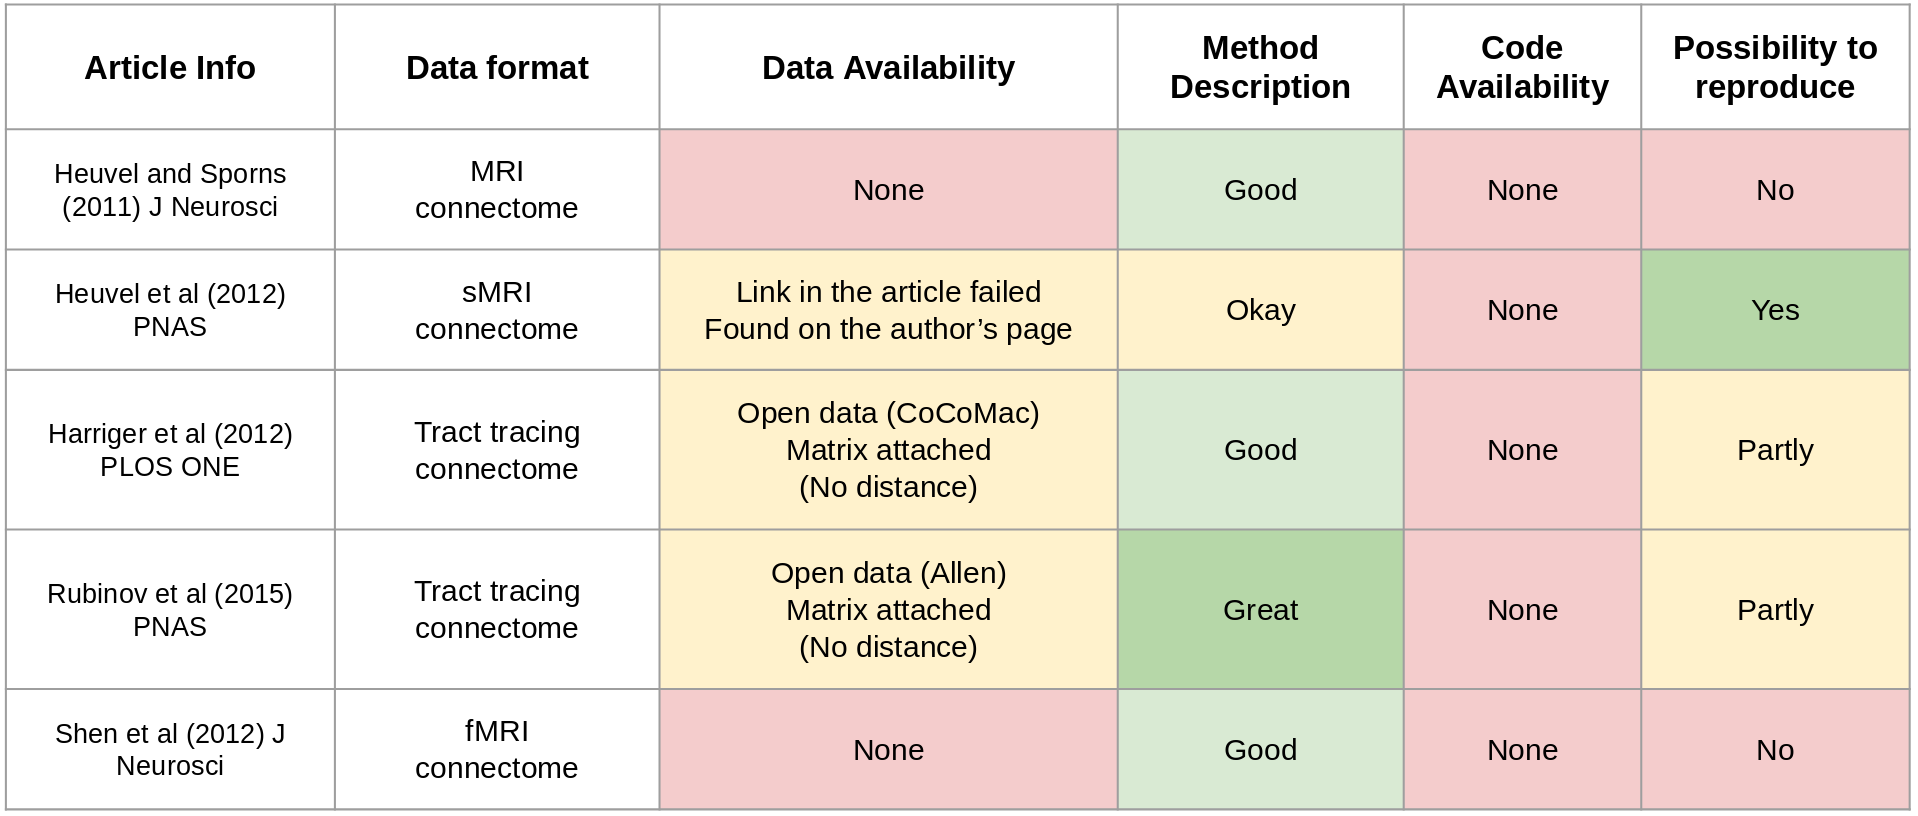
\includegraphics[width=1.1\textwidth,center]{table1}
  \caption{\textbf{Choosing project}}
  \label{fig:table1}
\end{figure}

\begin{figure}[!htp]
    \makebox[\linewidth][c]{%
        \begin{subfigure}[b]{0.5\textwidth}
            \centering
            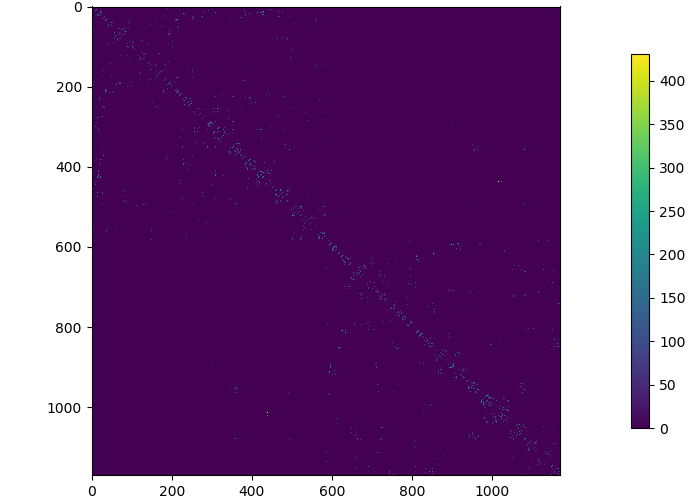
\includegraphics[width=\textwidth]{conn-1}
            \caption{}
            \label{fig:conn1}
        \end{subfigure}
        \begin{subfigure}[b]{0.5\textwidth}
            \centering
            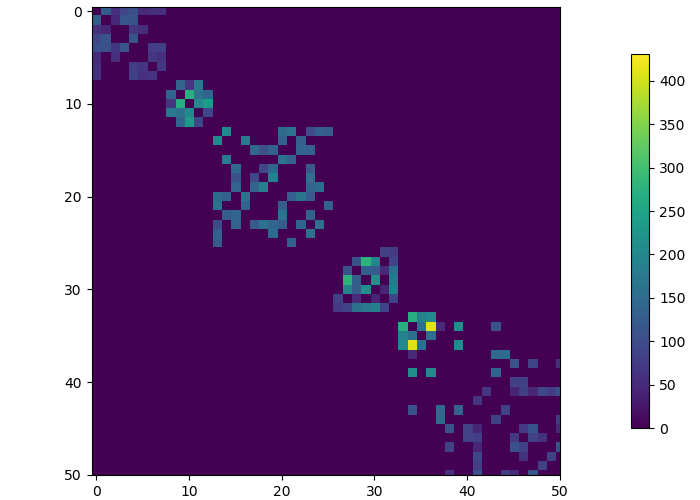
\includegraphics[width=\textwidth]{conn-2}
            \caption{}
            \label{fig:conn2}
        \end{subfigure}
    }
    \caption{\textbf{Connectivity matrix}: (a) the original (b) the first 50 dimensions.}
    \label{fig:conn12}
\end{figure}
\begin{figure}[!htp]
    \makebox[\linewidth][c]{%
        \begin{subfigure}[b]{0.5\textwidth}
            \centering
            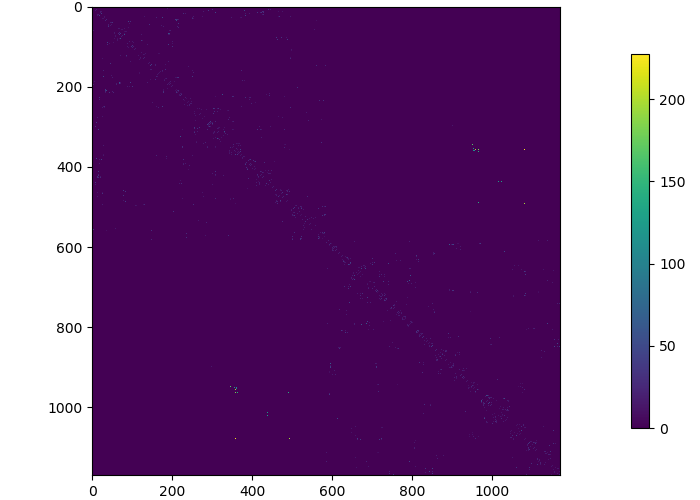
\includegraphics[width=\textwidth]{dist-1}
            \caption{}
            \label{fig:dist2}
        \end{subfigure}
        \begin{subfigure}[b]{0.5\textwidth}
            \centering
            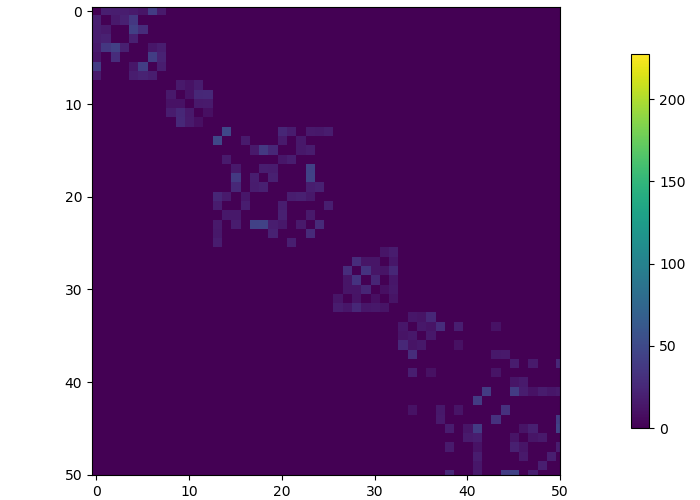
\includegraphics[width=\textwidth]{dist-2}
            \caption{}
            \label{fig:dist2}
        \end{subfigure}
    }
    \caption{\textbf{Distance matrix}: (a) the original (b) the first 50 dimensions.}
    \label{fig:dist12}
\end{figure}
\begin{figure}[!htp]
    \makebox[\linewidth][c]{%
        \begin{subfigure}[b]{0.5\textwidth}
            \centering
            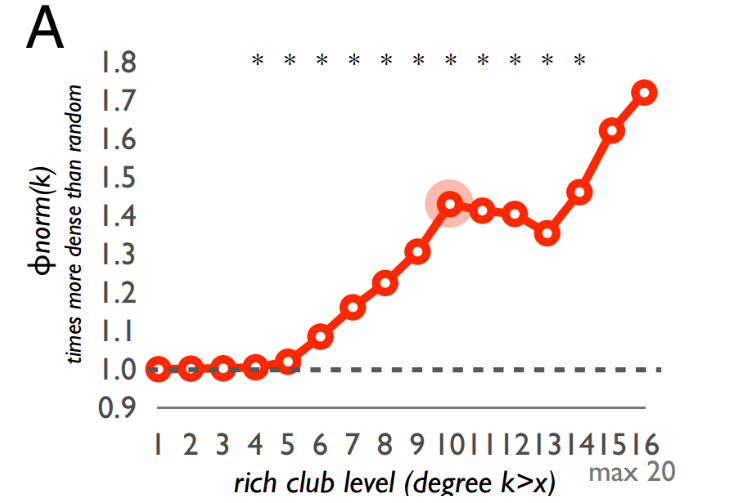
\includegraphics[width=\textwidth]{orig_fig1}
            \caption{}
            \label{fig:fig1}
        \end{subfigure}
        \begin{subfigure}[b]{0.5\textwidth}
            \centering
            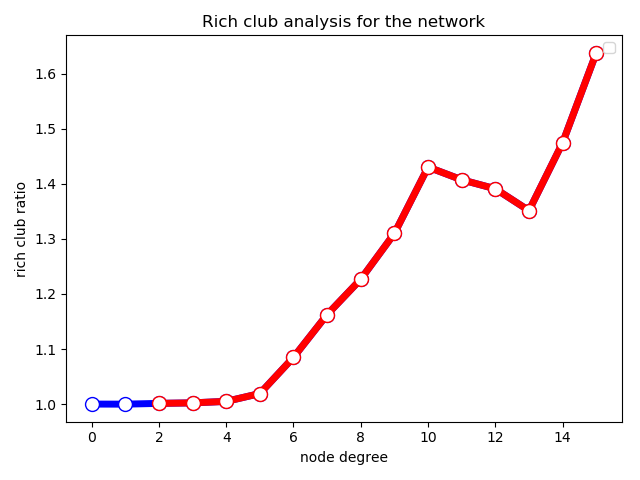
\includegraphics[width=\textwidth]{rc-1}
            \caption{}
            \label{fig:rc1}
        \end{subfigure}
    }
    \caption{\textbf{Rich club detection}: (a) the original (b) the reproduced result.}
    \label{fig:fig1}
\end{figure}

\begin{figure}[!htp]
    \makebox[\linewidth][c]{%
        \begin{subfigure}[b]{0.3\textwidth}
            \centering
            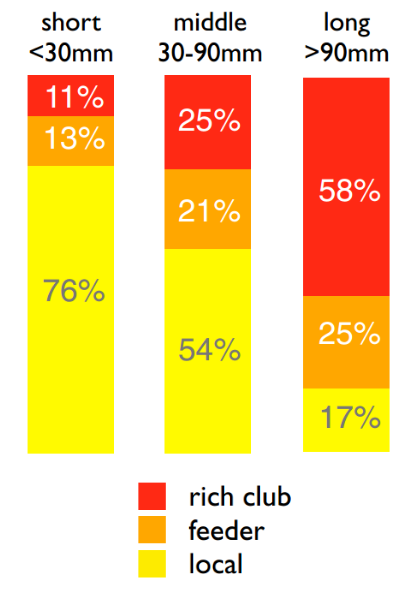
\includegraphics[width=\textwidth]{orig_fig2}
            \caption{}
            \label{fig:fig2-1-orig}
        \end{subfigure}\\
        \begin{subfigure}[b]{0.4\textwidth}
            \centering
            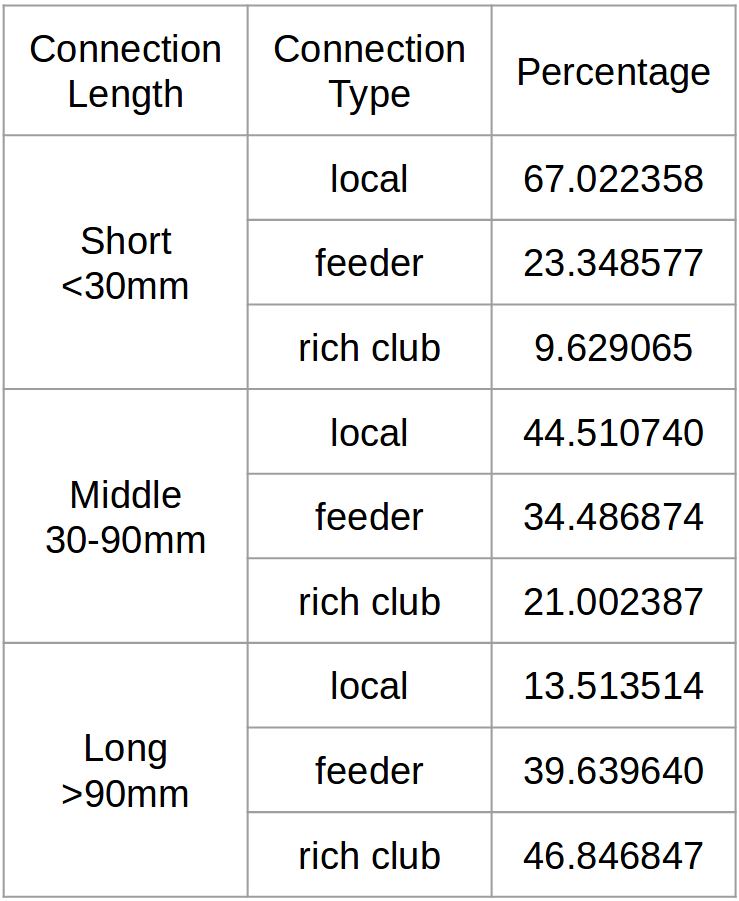
\includegraphics[width=\textwidth]{table2}
            \caption{}
            \label{fig:table2}
        \end{subfigure}
    }
    \caption{\textbf{Connection types grouped by length}: (a) the original (b) the reproduced result.}
    \label{fig:fig2-1}
\end{figure}

\begin{figure}[!htp]
    \makebox[\linewidth][c]{%
        \begin{subfigure}[b]{0.2\textwidth}
            \centering
            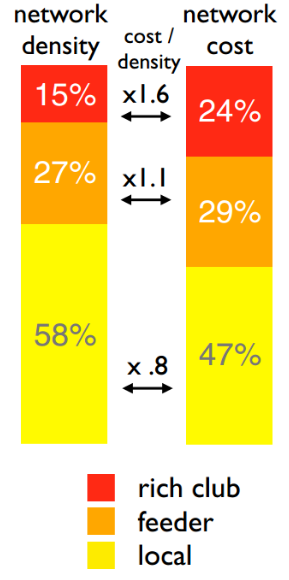
\includegraphics[width=\textwidth]{orig_fig3}
            \caption{}
            \label{fig:fig2-2-orig}
        \end{subfigure}\\
        \begin{subfigure}[b]{0.6\textwidth}
            \centering
            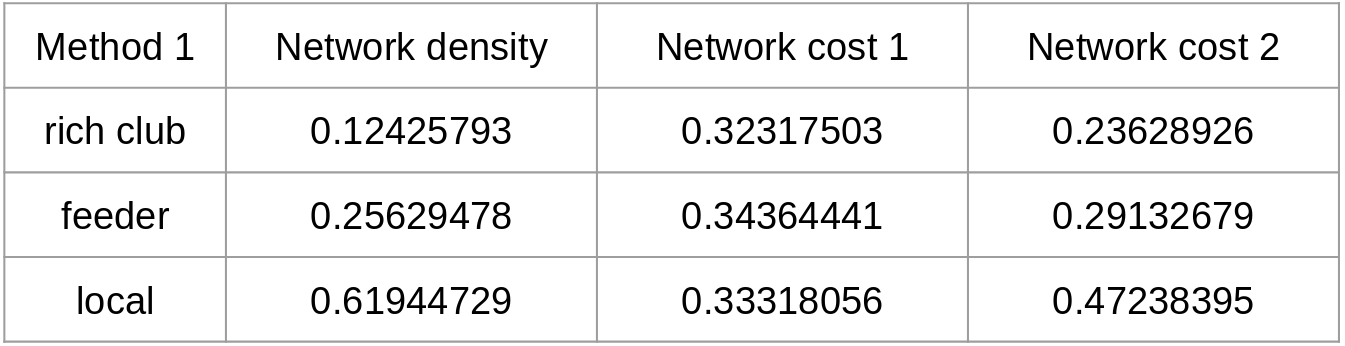
\includegraphics[width=\textwidth]{table3}
            \caption{}
            \label{fig:table3}
        \end{subfigure}
    }
    \caption{\textbf{Network density and communication cost}: (a) the original (b) the reproduced result.}
    \label{fig:fig2-2}
\end{figure}

\begin{figure}[!htp]
    \makebox[\linewidth][c]{%
        \begin{subfigure}[b]{0.35\textwidth}
            \centering
            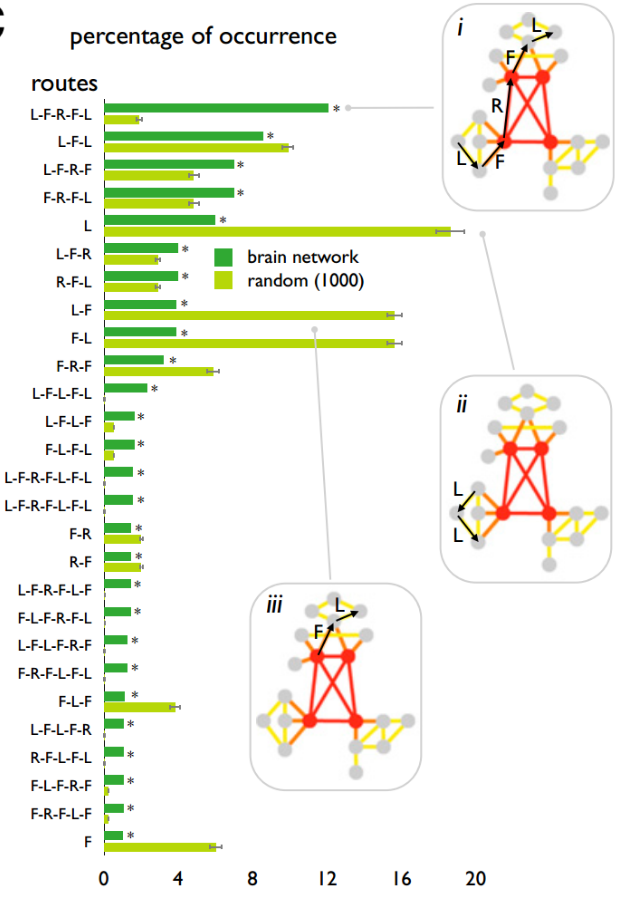
\includegraphics[width=\textwidth]{orig_fig4}
            \caption{}
            \label{fig:fig3-orig}
        \end{subfigure}
        \begin{subfigure}[b]{0.4\textwidth}
            \centering
            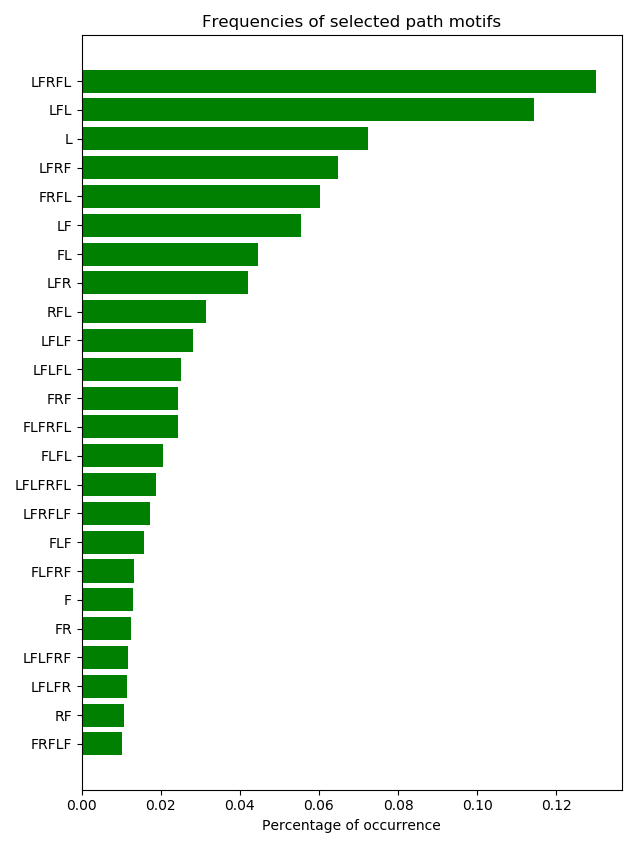
\includegraphics[width=\textwidth]{path-1}
            \caption{}
            \label{fig:path1}
        \end{subfigure}
        \begin{subfigure}[b]{0.15\textwidth}
            \centering
            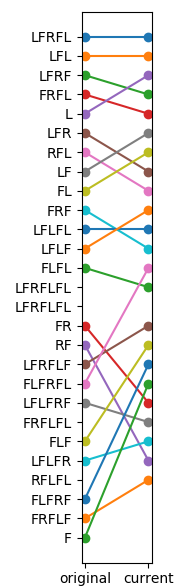
\includegraphics[width=\textwidth]{path-2}
            \caption{}
            \label{fig:path2}
        \end{subfigure}
        \begin{subfigure}[b]{0.15\textwidth}
            \centering
            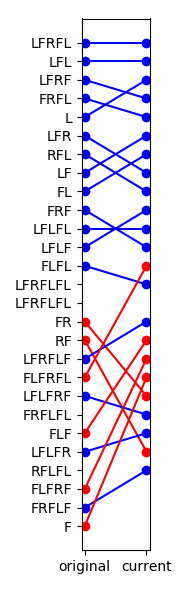
\includegraphics[width=\textwidth]{path-3}
            \caption{}
            \label{fig:path3}
        \end{subfigure}
    }
    \caption{\textbf{Path motifs}: (a) the original (b) the reproduced result (c) comparison of ranking (d) comparison of ranking (changes less than three ranks shown in blue)}
    \label{fig:fig3}
\end{figure}



\end{document}
